%!TEX root = ../thesis.tex

\graphicspath{{Chapter3/Figures/}{Chapter3/Tables/}{Chapter3/Charts/}}

\chapter{Methodology}

\section{Introduction} %Section - 3.1 

This chapter is divided into three sub-sections documenting the methodological approach to each of the key challenges in observing the impact of team factors through mining software repositories. As reflected in Figure ~\ref{fig:chapteroverview} outlining the structure of this chapter, these challenges are broadly in the categories of Definitions, Mining and Metrics. In order to begin to establish correlations between team factors and the internal attributes of FLOSS software, it is first necessary to define team size and stability and establish an empirical approach to their measurement. This is the topic of the first section in this chapter. The second section is concerned with the identification of an appropriately rich data set to study which, fortunately, open source repositories provide with few technical limitations. The criteria of selecting a forge to mine will be articulated and a mechanism to mine this data and extract information in a consistent, reliable and repeatable way is described. Finally, in its final section, this chapter details the approach to measuring the pertinent internal structural attributes of the code through the evolution of the project. 
 
\begin{landscape}
\begin{figure}[htbp!] 
\centering    
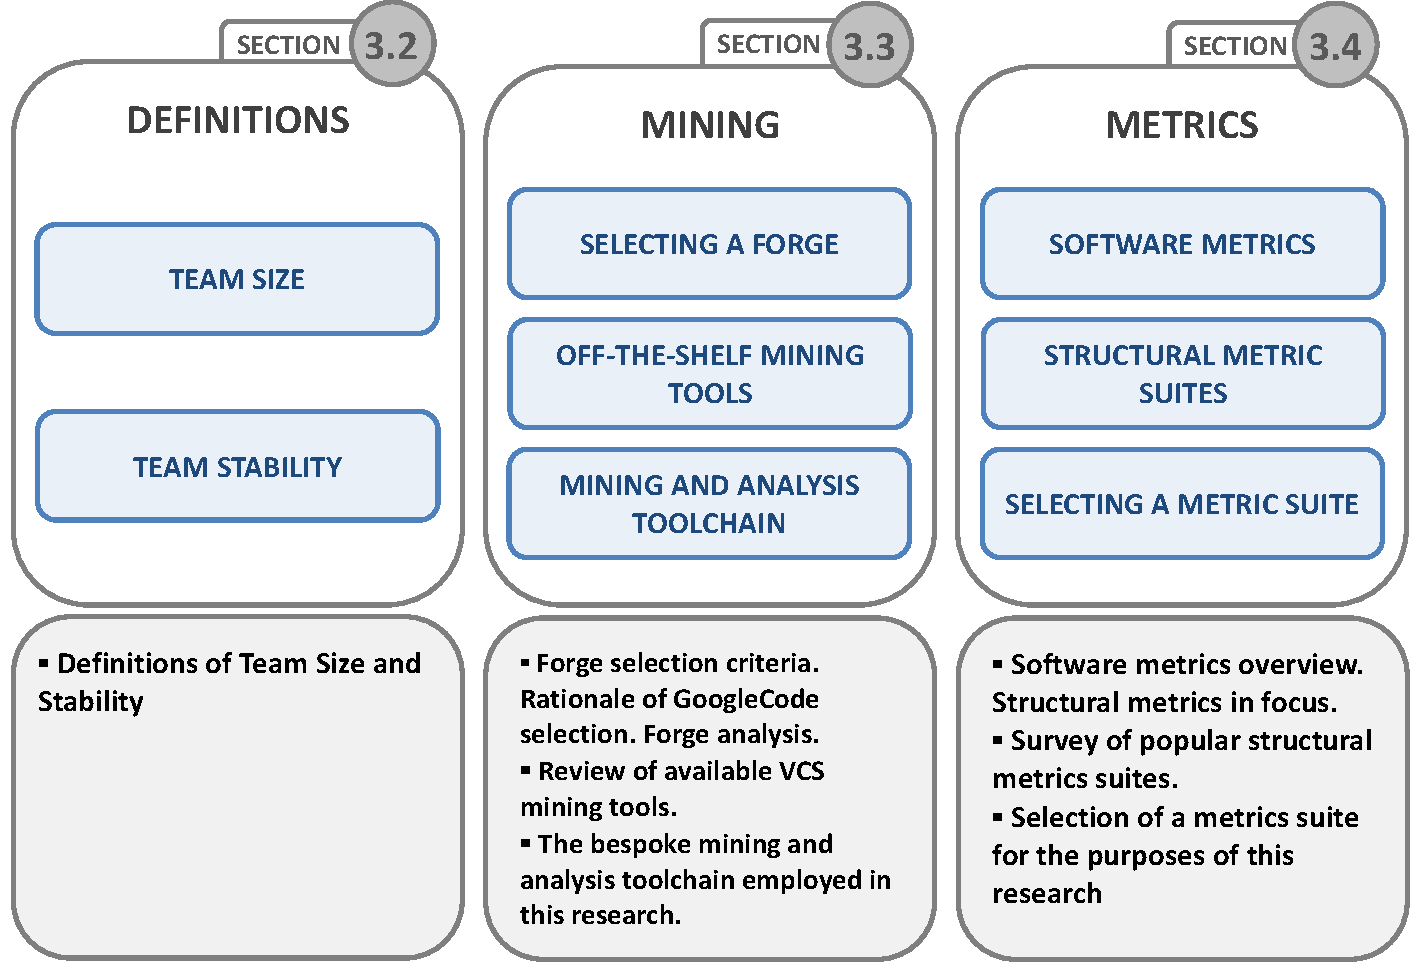
\includegraphics[width=1.1\textwidth]{ChapterOverview.pdf}
\caption{Chapter 3 outline providing an overview of the contents of each section.}
\label{fig:chapteroverview}
\end{figure}
\end{landscape}

\section{Definitions} %Section - 3.2
\subsection{Development team size}
There are a number of possible definitions of a software development team. Both Capra et al. and Smith et al. consider a team to consist of all developers to have worked on a codebase for any length of time \citep{capra2008framework, smith2001empirical} while Nagappan et al. \citep{nagappan2008influence} consider the development team to also include management, administration and operations personnel. Given the context of mining open source repositories, there is a preference to define team size as the cumulative total of all unique committers present in the revision history in the version control system of a given project. This definition is consistent with the prior art, simple to measure and reproduce, and elegantly enables the representation of the plurality of the unique development design approaches that may have influenced the evolution of a codebase. 

There are some potential limitations to this approach, most notably that we do not distinguish between frequent committers and causal (infrequent) committers. As will be discussed later in this thesis, while it is true that the majority of commit activity takes place by a minority of committers, the majority of committers do make a significant contribution and cannot be discounted, hence this is not regarded as a threat to validity. Similarly, when defining the team, the time during which developers contributed to the project is not considered. While it could be considered counter-intuitive that developers making contributions without any time overlap be considered part of a single team, analysis of the data sample shows that this is by far the exception in the GoogleCode forge, with the vast majority of developers making contributions in overlapping time windows with their fellow team members.

\subsection{Development team stability}
There has been relatively little empirical work that investigates the stability of development teams and its impact on aspects of the software development process. This could be due to the fact that it is a non-trivial task to capture a measure of stability. In the prior art, team stability is also referred to using the terms team fluidity or team familiarity \citep{huckman2009team} and care is taken to distinguish this concept from 'team tenure'- i.e. the cumulative programming experience of the individuals on the team \citep{hackman2002leading}. To measure team stability a similar approach to Huckman et al \citep{huckman2009team} is adopted, defining this as the cumulative time that each member has worked with every other member of the team. This approach is consistent with the limited prior art in this field and offers a simple, easily understood measure. Chapter 6 expands on this definition and proposes a methodology to calculate stability as it accrues within a project team.
	
\section{Mining} %Section - 3.3
\subsection{Overview}
Mining Software Repositories is a term that refers to the extraction, inspection, and analysis of artefacts produced through the software development process in order to deduce useful information about software projects. The intention is often to make this information available both to researchers to build upon and to industry practitioners to better inform decision-making \citep{hassan2008road}.

A software repository is built on a Version Control System (VCS), such as CVS \citep{cvs} or GIT \citep{git}, which is used to manage change in source code. These repositories come with a great deal of data that can be mined and subsequently analysed. Each act of file creation, deletion, or edit is represented within a 'commit'. Meta-data associated with every commit lists the paths of files that have been modified, committer details and a date. Snapshots of the source files themselves can be retrieved in their present state or at any point in their history - typically either for manual qualitative analysis or more often by machine-driven quantitative analysis. By mining software repositories, the evolution of software can be observed. 

Studying aspects of software engineering, and indeed social science, through the mining and subsequent analysis of data from FLOSS repositories is a well-trodden path with a large volume of academic studies leveraging this approach \citep{hassan2008road, hemmati2013msr}. There are a number of reasons why this approach is widely adopted:

\begin{itemize}
\item \textbf{Depth:} There are several million FLOSS projects available in the public domain - with thousands being added on a daily basis. Although a large number of projects never reach maturity \citep{comino2005planning}, this is still an extremely rich resource to mine\citep{deshpande2008total}.
\item \textbf{Access:} Under the GNU \citep{license2007version} license under which FLOSS projects are typically distributed, no restrictions apply to extracting, analysing, and publishing data derived from the publicly available source code or associated meta-data. In contrast, access to source code for proprietary commercial software is often restricted to the relevant in-house development team only for security, compliance and competitive reasons.
\item \textbf{Rich data:} Open source forges such GitHub \citep{github} or GoogleCode \citep{googlecode} come with a great deal of data that can be mined and analysed. In addition to the VCS commit data, there is also project level information that is made available including project categorisation, activity, artefacts, and bug reports. The FlossMole project \citep{howison2009flossmole} has worked to extract, normalise and make available project-level meta-data available across forges in unified format. Some of their artefacts are used in this research.
\end{itemize}

\subsection{Selecting a forge to mine}
There are a number of popular open source project hosts or 'forges'. According to research in 2011 (at the outset of this research's data collation activities) in terms of the number of commits, GITHub was the most popular, followed by SourceForge and then GoogleCode \citep{grady2011what}. Each of these forges attracts has a unique and varied make-up of languages making up its project population - see Table ~\ref{tab:LanguagePopularity}.

\begin{table}
\centering 
\captionof{table}{Popularity of languages in top 3 open source software forges (reproduced from Redmonk \citep{grady2011what})}
\begin{tabular}
 \centering 
 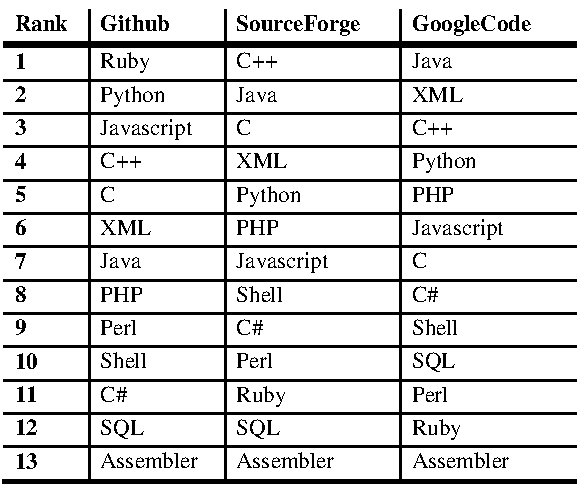
\includegraphics{LanguagePopularity.pdf}
 \label{tab:LanguagePopularity}
\end{tabular}
\end{table}


The practicalities of constructing a toolchain that is capable of mining data from a VCS and subsequently conducting static code analysis to extract the pertinent internal attributes of the software meant that it was going to require significant additional effort to accommodate more than one programming language. Given that one of the aims of this work is to maintain the relevance of this work to both the research and practitioner communities, it was logical to select a programming language with a high degree of popularity. For this reason, the Java was chosen as it consistently rates as the programming language with the highest adoption rates \citep{tiobe2017}. This also has the fortunate consequence of meaning that in most large forges there are a large number of Java projects available for study.  Furthermore, from a static code analysis tooling perspective, Java is very well supported.

GoogleCode was the open source forge selected for its popularity and high level of Java adoption rates. Another strong advantage in favour of GoogleCode was that they allowed project administrators to choose from among three available version control systems - Subversion, GIT, and Mercurial - on which to host their source code meaning that the mining toolchain would be sophisticated enough for others to reuse to mine GitHub (which uses GIT as it's underlying VCS) or SourceForge (which uses Subversion and Mercurial). This is helpful as it means that the toolchain developed for this research can have utility across a broad set of forges. This is particularly pertinent given that GoogleCode announced that it was shutting down their service and entering 'archival mode' - meaning that any future research on active projects will not happen on the GoogleCode forge. 

At this point it is also worth noting that, since the selection of the repository to study, the landscape has significantly changed and new repositories such as Assembla \citep{assembla}, and Gitlab \citep{gitlab} have established a strong presence - both of which use GIT as the underlying VCS - helpfully ensuring that the toolchain remains current.

\subsection{Overview of the GoogleCode forge}
As of May 2012, GoogleCode hosted 236,787 projects of which a significant number has seen sustained developer activity. GoogleCode projects are assigned 'labels' by the project administrators to assist in categorising the project. Many projects are 'forks' from popular projects - often where developers choose to take the project evolution in a slightly different direction or choose to 'experiment' on the codebase in their own sandbox. Forked projects retain the revision history of the original project which creates a challenge in ensuring that a forked project with a handful of commits isn't mistaken for the more popular parent project. As this is a particularly difficult challenge for which a unique solution was devised, a section is devoted to this topic later in this chapter.

The GoogleCode repository was started on the 27th of July 2006 \citep{shankland2006google} and the decision was announced nine years after its inception for its shut down \citep{dibona2006bidding}. This offers a unique opportunity to observe a forge throughout its lifespan. As we study commit patterns, it is notable in Figure ~\ref{fig:HistoricGoogleCodeActivityLevels} that the cumulative number of commits across all projects grows from the low hundreds at the forge initiation to a peak of over 10K commits per day. It is also notable that the committer activity begins to steadily tail off towards the end of 2010 as projects migrate to more popular repositories such as GitHub. In the first half of 2011 the commit activity on GitHub surpassed GoogleCode, SourceForge and Microsoft Codeplex combined \citep{redmonk2011}. This shift led industry commentators to observe that in 2011 GitHub had become the major centre of gravity within the open source space. This is likely attributable to the collaborative nature of its offering which pushed the boundaries of 'social coding' by providing transparency on contributors activity and allowing them further their skills and manage their reputation \citep{dabbish2012social}. As GitHub continued its exponential growth over the subsequent years, GoogleCode did not compete in a meaningful way enhancing or rebooting its offering. In this context, it is easy to rationalise Google's decision to shut down the repository, closing the forge to new project creation in 2015.
 
\begin{figure}[htbp!] 
\centering    
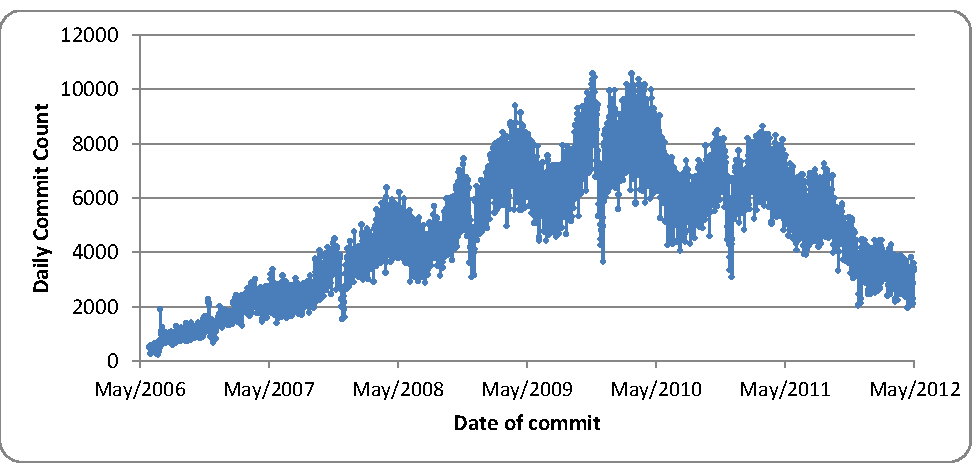
\includegraphics[width=1.0\textwidth]{HistoricGoogleCodeActivityLevels.pdf}
\caption{Commit histogram showing daily activity levels across the entirety GoogleCode.}
\label{fig:HistoricGoogleCodeActivityLevels}
\end{figure}

In the data analysis and visualisations throughout this thesis a fixed upper bound is defined for the time period of study. This was necessary as mining such large volumes of data can take multiple weeks to successfully extract. The majority of this data mining effort took place in the years 2012-2013 and for this reason, it was chosen to only study data up to the end of May 2012. This date was also chosen as it coincides with the availability of then up-to-date FLOSSMole artefacts which, as outlined later in this chapter, facilitates the data mining effort.  

Figure ~\ref{fig:HistoricGoogleCodeActivityLevels} gives an indication of the activity trends but doesn't give an insight into whether this is down to an increase in the number of projects or whether this is attributable to greater activity on existing projects. Figure ~\ref{fig:ProjectCreationHistogram} helps establish that this commit activity is, indeed, visually correlated with an increasing number of projects. Clearly observable is an initial spike of project creation on the go-live date of GoogleCode. In October 2011, a significant drop in project creation is evident, decreasing to an average rate of 3 projects per day. There is no immediately obvious reason in the publicly available records to explain this drop but it is clear that, even prior to this drop, there was a general downwards trend.

\begin{figure}[htbp!] 
\centering    
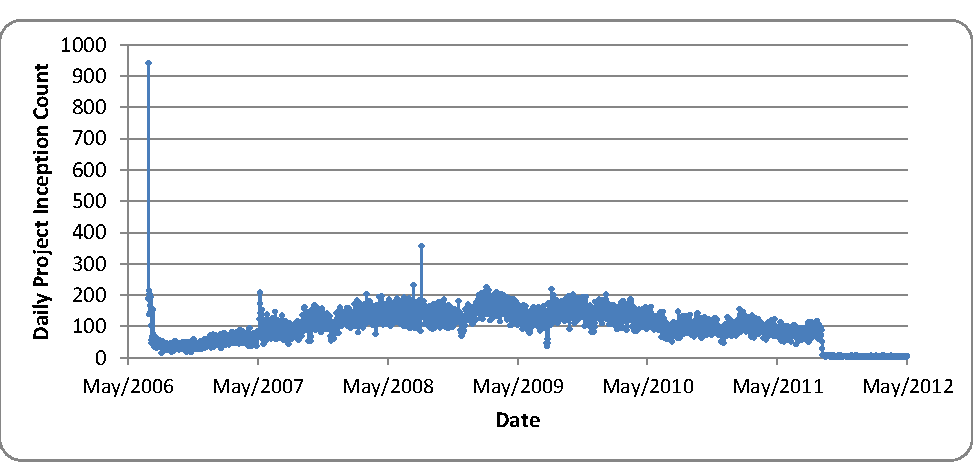
\includegraphics[width=1.0\textwidth]{ProjectCreationHistogram.pdf}
\caption{A histogram depicting the daily rate of new project creation.}
\label{fig:ProjectCreationHistogram}
\end{figure}
	
From a total project count of 236,787 only 95,490 have a single commit (corresponding to the initial project creation). 			

\subsection{Toolchain requirements}
This research presented a number of challenges to mine the commit details for all the projects in GoogleCode's repositories and consolidate this information within a single data model and, ultimately, in a relational database for further analysis. 

Given that this research tackles the study of team stability, it is necessary to mine the entirety of the chosen repository in order to derive team stability analytics based on the number of times each committer has worked with every other committer. This research clearly does not stop at an analysis of commit data. Given the focus on the internal attributes of software it is essential to inspect the source files for each project chosen for study, from which structural metrics can be extracted. This data, when juxtaposed with the relevant commit data, allows the trends surrounding structural metrics to manifest as projects evolve and mature. Given the sheer size of GoogleCode this is no small task and it will involve hundreds of gigabytes of data transfer, multiple gigabytes of storage and many days of processing to produce an accurate representation of individual contributor behaviour.

The requirements of the toolchain can be articulated as follows.
\begin{itemize}
\item \textbf{Mine VCS logs and software metrics} Mine VCS revision history and conduct static source code analysis against each snapshot of source code.
\item \textbf{Breadth and scale} Capability of mining revision history of thousands of repositories across SVN, Mercurial and GIT.
\item \textbf{Queriable data sets} Store revision history in normalised queriable form.
\item \textbf{Joinable data sets} Join VCS revision history data with software metrics mined from snapshots of source code.
\end{itemize}

\subsection{Open Source Tools}
Table ~\ref{tab:VCSMiningToolSummary} provides an overview of several relevant open source mining tools - Softchange \citep{german2004mining}, Hipikat \citep{vcubranic2003hipikat}, Dynamine \citep{livshits2005dynamine}, Kenyon \citep{bevan2005facilitating} and CVSAnaly \citep{robles2004remote} - along with a brief summary of their limitations with regards to this research.

\begin{table}
\centering 
\captionof{table}{A comparison of a number of version control mining tools}
\begin{tabular}
 \centering 
 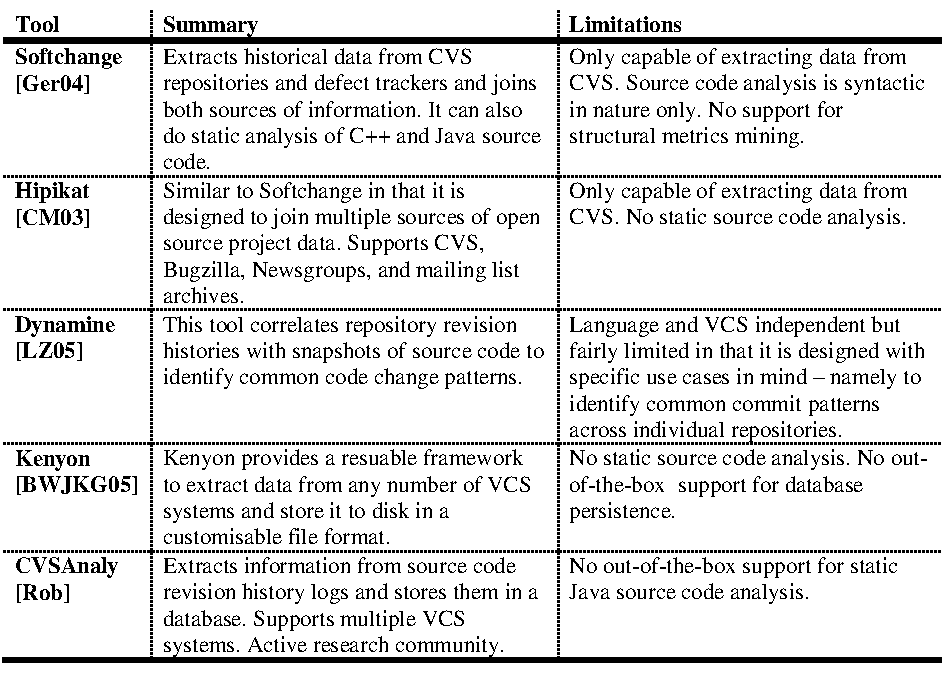
\includegraphics[width=1.0\textwidth]{VCSMiningToolSummary.pdf}
 \label{tab:VCSMiningToolSummary}
\end{tabular}
\end{table}

Of these tools CVSAnaly was deemed the more versatile to mine, normalise, and store revision history. The main functional limitations associated with CVSAnaly in the context of this research are as follows.

\begin{itemize}
\item \textbf{Missing support for the Mercurial VCS:} This is one of the GoogleCode supported VCS systems alongside GIT and Subversion - both of which are supported by CVSAnaly.
\item \textbf{Missing support for Static Code Analysis:} Although there was no out-of-the-box support for Java static code analysis, there is support for 'extensions'. For this approach to be successful, such an extension would need to check-out each version of the codebase, execute static code analysis, and commit the results to a version of the CVSAnaly schema.
\item \textbf{Restricted Database Schema:} Integrating static code analysis would necessitate further building out the CVSAnaly schema to store the mined metrics 
\end{itemize}

Consideration was given to committing to enhancing CVSAnaly with the aforementioned functionality - an undertaking that would require that the CVSAnaly codebase be sufficiently understood in order to correctly identify the integration points for various new functionalities. However, given the limited functional scope and the authors lack of familiarity with Python, the language that CVSAnaly extensions must be programmed in, the balance ultimately tipped in favour of creating a bespoke toolchain for data mining. 

\subsection{Toolchain}
This section documents the toolchain developed to mine and analyse the GoogleCode forge. Particular attention is devoted to those components that are common to both team size and team stability analysis; those components that are particular to either type of analysis are discussed in chapter 4 and chapter 5 respectively.

\begin{figure}[htbp!] 
\centering    
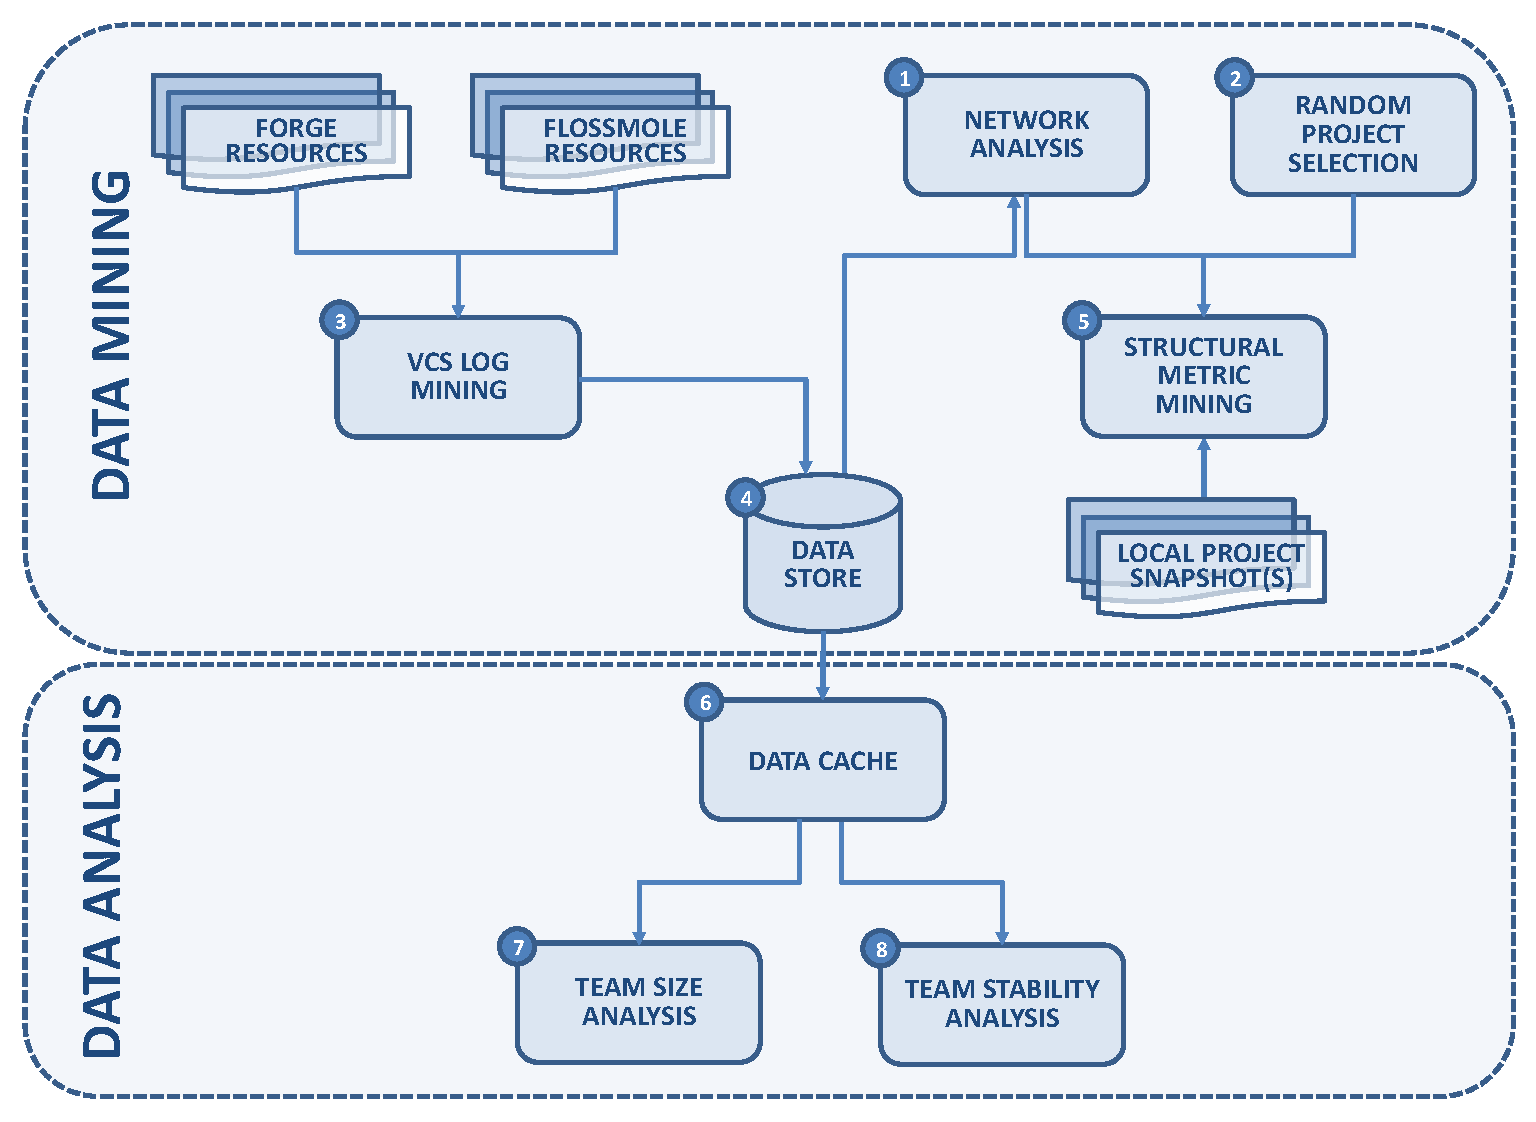
\includegraphics[width=1.0\textwidth]{Toolchain.pdf}
\caption{Toolchain to mine and analyse the GoogleCode forge.}
\label{fig:Toolchain}
\end{figure}

\begin{itemize}
\item \textbf{1. VCS Log Mining:} The FLOSSmole project makes available the raw data describing, at a project level, details about all projects hosted in GoogleCode. This, along with the GoogleCode project webpages and the associated repositories formed the input into the bespoke toolchain illustrated in Figure ~\ref{fig:Toolchain}. At its essence, the VCS mining component is a collection of shell scripts, run on a UNIX platform and driven by the FLOSSMole flat files and the GoogleCode project webpages, designed to retrieve, parse and persist the full revision history of all the projects in the forge. To mine this data, these scripts access all project repositories in the forge to retrieve the full revision history, parsing it accordingly and storing it in the database to then drive subsequent analysis. 

These scripts support three version control systems; Subversion, GIT, and Mercurial. In the case of Subversion and GIT, the revision history can be directly queried through the appropriate binaries (albeit through different syntax and requiring individual log parsers) while in the case of Mercurial it is necessary to clone the repository before retrieving the history. The revision history extraction scripts use the repository URL to determine the type of version control system and extract the data appropriately. 

\item \textbf{2. Network Analysis:} The network analysis conducted in this research is focused on accurately mapping committer activity and project engagement in the context of the activity of the broader development team. This is used to calculate the stability of a team through the evolution of the project as well as understanding the change in team composition from one project to the next. This analysis also enables the mining of the full data set for projects that fulfil the criteria necessary for team stability analysis; for instance, pairs of projects where the development team remained stable. This will be discussed further in chapter 5 as the team stability analysis is detailed.

\item \textbf{3. Project Sampling:} This is a Java component designed to extract, in a reproducible fashion, a representative sample of projects from the full data set of 236,787 projects in the GoogleCode forge. There is functionality to identify and select projects programmed in a particular programming language (Java) to simplify structural metrics mining. This component is covered in detailed in Section 4.2 of the next chapter.

\item \textbf{4. Structural Metric Mining:} This component comprises of, again, UNIX shell scripts responsible for checking out each version of the project, handing over the heavy lifting of metrics generation to an out-of-the-box metrics generation tool. Using an existing tool for structural metrics mining was favoured over writing a bespoke tool given that, unlike VCS mining, metrics calculation is complex and potentially error prone. This meant that creating a bespoke tool would require significant build and validation effort. Fortunately the landscape of available tools was sufficiently rich such that a suitable tool could be identified with ease and without the need for extensions or enhancements. Table ~\ref{tab:MetricMiningToolSummary} shows a comparison of the available metric generation tools categorised by the distribution license (commercial or open source) and deployment (standalone or integrated into an IDE). 'Understand' by Scientific Toolworks Inc. was chosen as it is amongst the most reputable and widely adopted, was available on academic license, and offers a command line tool that generates metric reports in an easily parsable format. The report created by Understand is then passed through a Java Parser which extracts the information that is pertinent to this research and stores it in a format appropriate to the metrics analysis component. The calculations used by Understand to generate metric values are in Table ~\ref{tab:Understand}.

\begin{table}
\centering 
\captionof{table}{A comparison of a number of structural metrics mining tools}
\begin{tabular}
 \centering 
 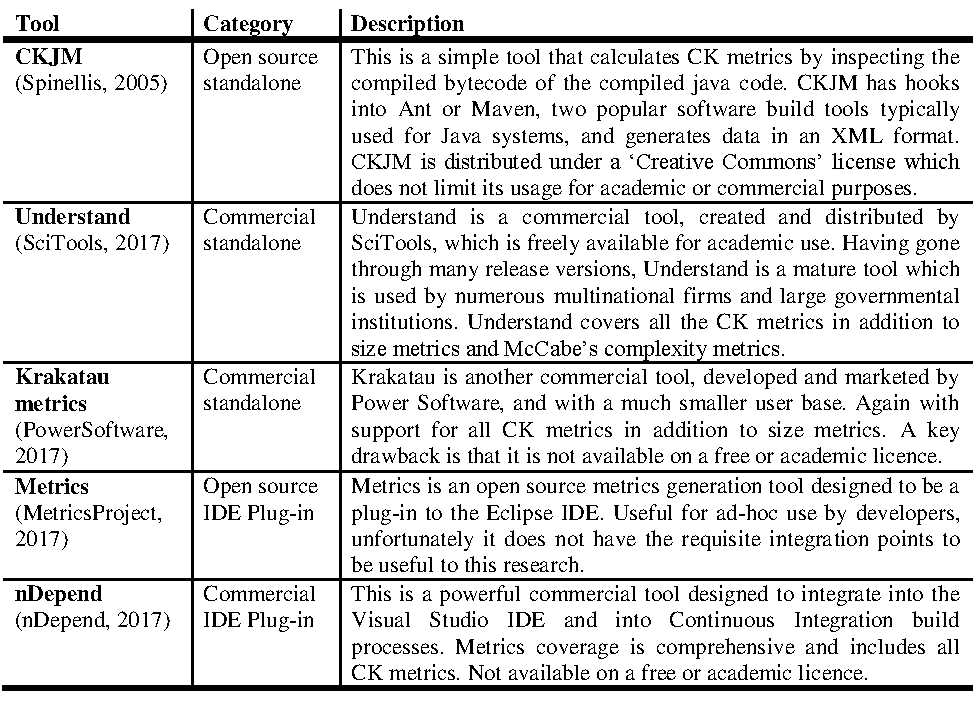
\includegraphics[width=1.0\textwidth]{MetricMiningToolSummary.pdf}
 \label{tab:MetricMiningToolSummary}
\end{tabular}
\end{table}

\begin{table}
\centering 
\captionof{table}{A description of how CK Metric values are calculated for Java classes by Understand.}
\begin{tabular}
 \centering 
 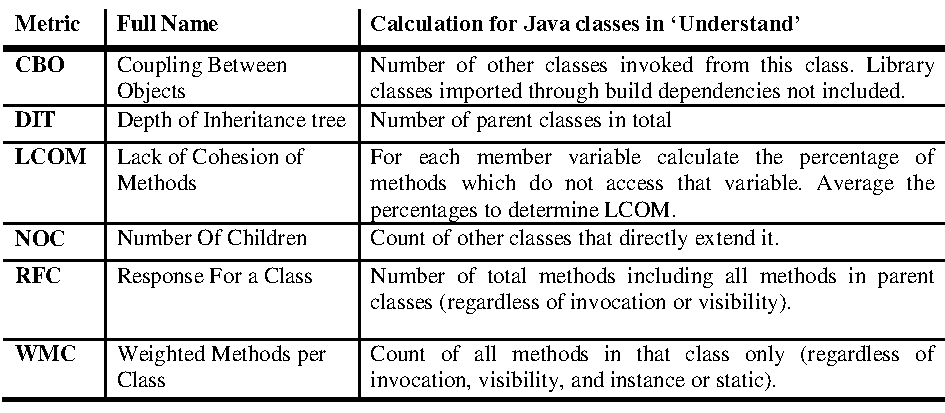
\includegraphics[width=1.0\textwidth]{Understand.pdf}
 \label{tab:Understand}
\end{tabular}
\end{table}

\item \textbf{5. Data Store:} Raw metrics and analysis should be stored in a queriable format to facilitate further data analysis - particularly statistical analysis - to identify trends and correlations. A MySQL database was created with a schema reflecting the data model outlined in Figure ~\ref{fig:Schema} to store the results of the VCS log mining and the structural metric mining. 
 
 \begin{figure}[htbp!] 
 \centering    
 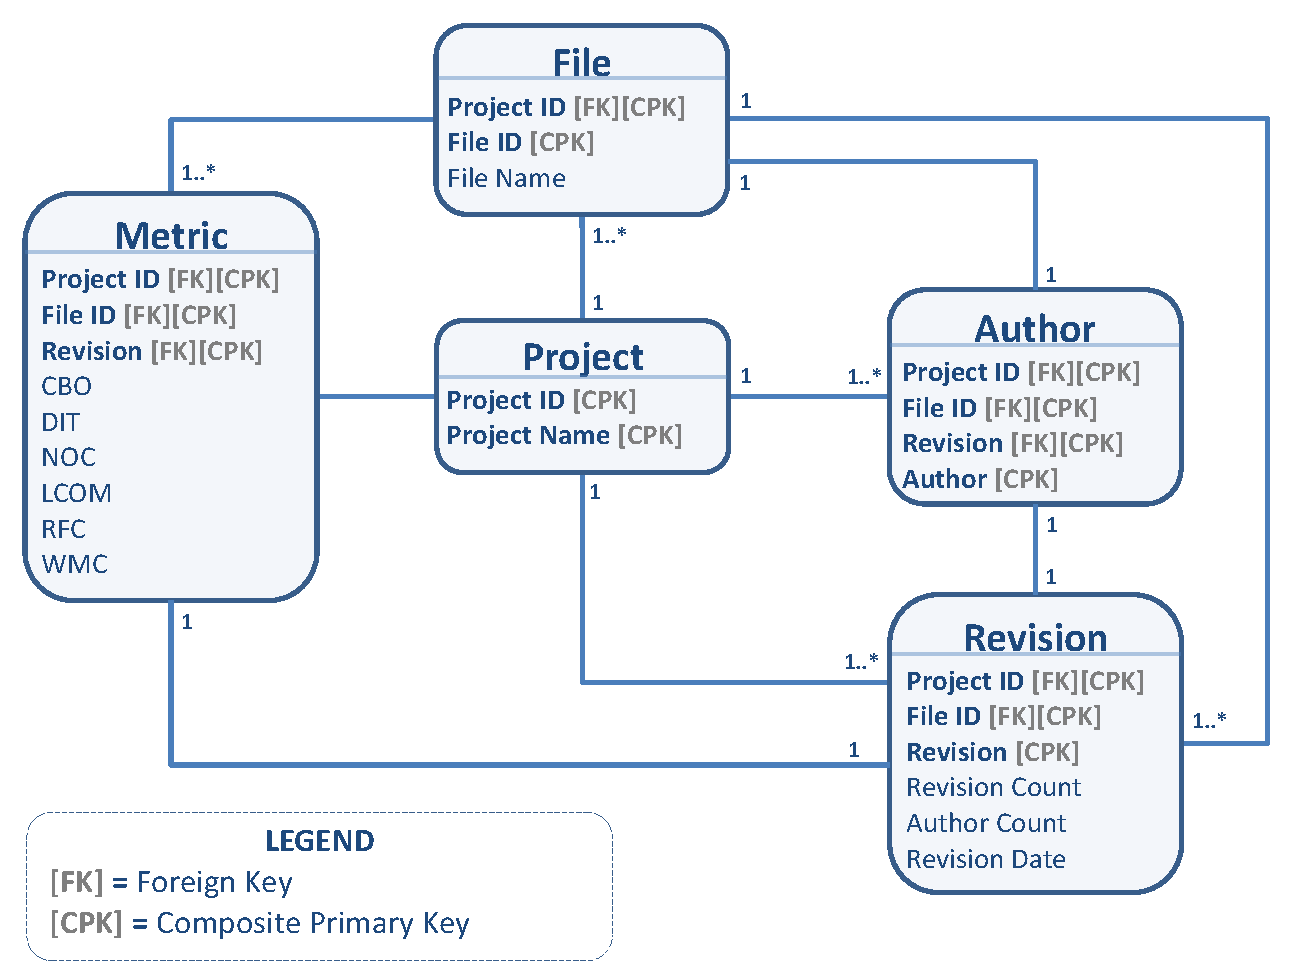
\includegraphics[width=1.0\textwidth]{Schema.pdf}
 \caption[A simplified ER diagram depicting the logical data model used by the data store.]{A simplified ER diagram depicting the data model used by the data store. This is closely reflected by the object model underpinning the analysis components.}
 \label{fig:Schema}
 \end{figure}

\item \textbf{6. Data Cache:}
When conducting analysis - and in particular network analysis - it is necessary to traverse a large data set multiple times in order to make meaningful observations on the data.

For example, to establish which committers have common project engagements, it is necessary to traverse the data set and categorise project engagements by committer. To calculate the stability of a team within a project, a traversal of the data for that project is required to determine the overlapping committer engagement periods. For this reason, it is efficient to load entire commit data into an in-memory data structure within the Java Virtual Machine running the team size and stability analysis to facilitate rapid access and flexible indexing. In practice this is implemented using HashMaps keyed by author and project as appropriate for the requisite type of analysis. 

\item \textbf{7. Team Size Analysis:} This is the subject of chapter 4 so will not be discussed at length here. However, as a brief overview it is worth mentioning that this is a Java component, connecting into the database and, at the heart of this analysis is joining structural metrics with commit level information in order to categorise and bucket metrics in a way that enables statistical comparisons between differing team sizes.

\item \textbf{8. Team Stability Analysis:} Similarly, this analysis is the subject of chapter 5 but suffice to say that the design is similar to the previous component with a focus on reading commit data and its associated meta-data to calculate team stability measures. This then drives the categorisation and statistical comparison of structural metrics in order to ascertain the impact of stability on metric values.
\end{itemize}

\subsection{Validating the Toolchain}
One challenge involved in developing a bespoke toolchain was the requisite effort to ensure its validity. Whenever writing code, typically good engineering practices such as ensuring adequate unit test coverage should be a given. The approach taken to development of components for this research was no different. This gives confidence that individual elements in the toolchain have been correctly implemented. 

However, to get confidence that our complete toolchain is functionally sound from an end-to-end perspective, it was necessary to run it against a small project for which metrics had been manually calculated as a reconciliation point. To ensure that the validation process was not overly taxing yet suitably thorough, the project to validate was chosen to have a limited number of project revisions yet have multiple authors including multiple revisions and authors on the same source file. The project selected for this purpose was zsea-planetwars as it has 8 revisions and 3 authors. The project was downloaded in each of its 8 snapshot states and imported within the Eclipse IDE. For each file within each snapshot, the metrics were derived by hand and validated successfully.

\subsection{Toolchain Performance}
The toolchain uses standard programming languages and does not require any specialised hardware or operating systems. However, as mining processes are network bandwidth intensive, the software was deployed to a commercially hosted Virtual Private Server (VPS) as this guaranteed faster internet connectivity than could be achieved with a typical domestic connection. The VPS account was an entry-level single core deployment with 512MB RAM, 25GB of data storage. The Linux distribution was CentOS 6.8.

The time taken to download VCS logs is dependent on the volume of revision history for a given project but is generally in the single digit seconds. Mining structural metrics is a more time-consuming process and can take around several minutes for a single 'snapshot' of the source code. This is a roughly equal distribution between the time taken to download the source code and the time taken to run static code analysis. Medium sized projects can have hundreds of revisions which leads to a total analysis time in the hours. As a rough guide, mining structural metrics for a 1000 project sample takes about 300 hours. Even with the limitation of a single core, this process can be made much faster by running parallel processes (multi-threading). 25 threads was found to be optimal and resulted in a sample processing time of approximately 24 hours.

Once stored in the MySQL relational database the data associated with all revisions of a single project within the sample takes up approximately 4-5MB of disk space. While this may present a minor technical when mining the entirety of the forge for structural metrics, this was not a concern when limiting the static analysis to a representative sample of projects.

\section{Metrics} %Section - 3.4
\subsection{Overview}
While ISO/IEC 25010 recognises that internal quality drives external quality, it does not offer any specific direct measures for internal quality but instead offers a framework to define metrics that are influenced by internal quality. For example, maintainability is measured by the resources expended to modify software. These measures are neither direct nor predictive. Fortunately, there has been significant research in formulating such direct measures. 

Coleman et al \citep{coleman1994using}, in the early 90s, developed a maintainability model that used static measures of source code to produce a percentage figure on how easy  a system is to support and change derived from a blend of measures including complexity metrics. This metric is still used today within Visual Studio \citep{msdn2015code} which classifies ranges which correspond to High, Moderate and Low maintainability. Heitlager et al \citep{heitlager2007practical} from the Software Improvement Group (SIG) critiqued this model as presenting difficulties in re-constructing the root causes that drive a particular measure and suggested an alternative maintainability model which blends structural metrics including complexity, volume, and unit size to drive its metrics. The strength in the SIG maintainability model is the simplicity with which a calculated index would be mapped to its constituent structural attributes.

In a similar vein, the approach of this research to observing indicators of internal quality is to directly measure the internal structural attributes of a codebase and draw upon established models to ascertain if the trends observed indicate enhanced or degraded internal software quality.

There are two primary categories of internal attributes of software - size and structure. Software size is a broad term and measurements can vary from basic line of code counts through to function-point analysis. It is tempting to assume that size is directly correlated to external attributes of fault-proneness and development effort while negatively correlated to maintainability \citep{akiyama1971example}. However, as Fenton states \citep{fenton2014software}, experience shows that this is not a valid assumption and that the structural attributes of software play a vital part in driving these external attributes.
 
This section first discusses the metrics which can be used to capture structural attributes followed by a brief historical context. The metric suite chosen for the purposes of this research is then discussed and detail is given to how previous research has linked these metrics to external quality attributes.

\subsection{What Are Structural Metrics?}
Software metrics embody an empirical approach to software engineering and are primarily designed to assist in making assessments of software artefacts and development processes, in the process guiding engineers and project managers in their decision making. A software metric is the quantitative measure of the degree to which a component, system, or process possesses a given characteristic or attribute \citep{ordonez2008state}. If used appropriately, software metrics can lead to a significant reduction in costs of the overall implementation and maintenance of the final software product. 

Structural metrics are a specific category of software metrics that allow us to measure and express the adherence of a codebase's structural attributes to sound engineering design principles. The key attributes in Object Oriented Programming are the interlinked concepts of coupling, cohesion, complexity, and modularity. These are explained as follows.

\begin{itemize}
\item \textbf{Coupling:} This is the degree to which components within software systems are interdependent. A high degree of coupling in a set of components implies that changes in one component may impact the other components in that set \citep{parnas1972criteria}. At a relatively low level, modern object-oriented languages provide paradigms (such as interfaces) to facilitate lower coupling between classes. Interfaces allow a developer to separate the method of interaction into a component from the implementation of functionality. At a higher level, enterprise design patterns such as the Service-Oriented Architecture facilitates lower levels of coupling between applications. Lower levels of coupling are desirable at each level of an enterprise software system \citep{pressman2005software} \citep{chidamber1998managerial}.

\item \textbf{Cohesion:} Cohesion is a measure of the extent to which functionality within a single component belongs together. A component that exhibits a high degree of cohesiveness typically encapsulates a single set of highly related functionalities. In object-oriented languages, a high degree of cohesiveness is a desirable trait and is consistent with the 'single responsibility principle' which states that a class should have a single purpose and its functionality should be encapsulated within the class - i.e. not exposing its inner workings to other components\citep{fenton2014software}. A high degree of cohesiveness and encapsulation is correlated with a low level of coupling \citep{chidamber1998managerial}.

\item \textbf{Complexity:} In the context of structural metrics, complexity refers to the structural complexity of software rather than the functional complexity. This is a contrast that will be discussed in the coming chapter in Section 4.5.3. Structural complexity is a measure of the degree of interactions between components in a software system \citep{fenton2014software}. A highly complex system would contain a large number of components and a large number of interactions between the components. Although the number of interactions between components is a driver of structural complexity, the nature of the interaction between two components can introduce further structural complexity if there is a dependency on the inner workings of the components (i.e. poor encapsulation and high coupling). Although functional complexity can often introduce structural complexity, all things being equal, lower measures of structural complexity are desirable.

\item \textbf{Modularity:} This refers to the extent to which a system's functionality is logically partitioned into independent components \citep{parnas1972criteria}. A high degree of modularity is desirable as it encourages low coupling and high cohesion which, in turn, reduces structural complexity \citep{parnas1972criteria} \citep{sullivan2001structure}.
\end{itemize}

\subsection{Survey of Metrics Suites}
There are a number of structural metric suites that commonly appear in both academic literature and practitioner tools. In this section a comparative survey is provided for the most popular metric suites and justification is given to the choices in this research. The discussion is limited to object-oriented structural metrics given that, as mentioned earlier in this chapter, this research studies Java software only. This is to the exclusion of suites such as the Halstead metrics. Furthermore, consideration is only given to those metric suites that comprehensively cover the key internal structural attributes - coupling, cohesion, complexity and modularity - to the exclusion of, for example, the McCabe metrics with their almost exclusive focus on structural complexity \citep{mccabe1976complexity} \citep{mccabe1989design}. For a fuller survey of the available object-oriented structural metric suites, the reader is encouraged to review the work of Gomathi et al \citep{gomathi2013an} and Xenos et al \citep{xenos2000object}. The comparison is therefore limited to the Chidamber and Kemerer suite, the MOOD metric suite, and the Lorenz and Kidd metric suite.

\begin{itemize}
\item \textbf{Chidamber and Kemerer metric suite} The Chidamber and Kemerer (CK) metric suite is one of the most cited of all structural metric suites within the academic community \citep{pressman2005software} with a great deal of research spanning the two decades since its creation. 

The CK metric suite is designed to operate on the most fundamental unit in object-oriented systems - the class. The CK metric suite contains measures that capture complexity, coupling and cohesion. The values of the measures are fairly arbitrary and there has been research into defining the thresholds that could indicate classes which would be more likely to require remedial action \citep{rosenberg1998applying}. While there has been some doubt cast on the theoretical and empirical validity of one of the measures in the suite \citep{fenton2014software}, nonetheless, this remains the most validated OO metric suite available \citep{kitchenham2010s} with a great deal of research successfully correlating the metrics to external quality attributes \citep{rosenberg1998applying, el2001prediction} \citep{basili1984software, subramanyam2003empirical}. This suite is covered in more detail later in this chapter.

\item \textbf{MOOD metric suite} The MOOD metric suite was developed by Brito e Abreu and Carapu\c{c}a in 1994 to provide system-level measures (as opposed to class-level measures) for object-oriented systems in order to guide and assess OO design quality \citep{abreu1994object}. The measures capture a broad range of structural attributes including encapsulation and polymorphism factors - factors absent from the CK metrics suite. In contrast to CK metrics where the values of the measures are arbitrary, the MOOD metric values are probabilities with values from 0 to 1 representing the likelihood of the existence of a particular attribute. Harrison et al conducted research detailing the utility of MOOD metrics to practitioners \citep{harrison1998investigation} finding that they present information that would be of general use to software managers to understand the overall attributes of a system. MOOD metrics are not widely adopted in academic research nor industry and this is reflected in the very scarce availability of tools that generate these metrics with Project Anaylzer \citep{abounader1997data} being the only distributed tool that the author could find. This tool only had support for the Visual Basic programming language. In its favour there has been significant research analysis which largely validated the MOOD metric suite \citep{abounader1997data, harrison1998evaluation}.

\item \textbf{Lorenz and Kidd metric suite} In their book object-oriented Software Metrics \citep{lorenz1994object} Lorenz and Kidd proposed a metric suite consisting of eleven metrics that, in a similar fashion to the CK metric suite, measured attributes at a class level. Metrics are broadly in four categories - size, inheritance, class internals (attributes that can be measured on a class in isolation such as cohesion) and class externals (attributes that capture how a class interacts with other classes such as coupling and reuse). Lorenz and Kidd also propose threshold values to help interpret metric observations. The Lorenz and Kidd suite did experience a degree of recognition in academic circles with a large number of citations \citep{nesi1998effort} but, with few validation studies \citep{sharma2012metrics} and no available tools to measure these metrics, it is fair to say that this metric suite has not experienced significant academic or practitioner adoption. This may be due to the fact that the metric suite is fairly basic and constitutes directly measurable attributes such as Number of Methods, Number of Public Variables and Number of Variables which has caused some doubt to be cast on its usefulness \citep{harrison1998investigation}.
\end{itemize}

\subsection{Choosing a Metrics Suite} The research questions in this thesis mandate a number of key criteria of the metric suite chosen for this work. The first main requirement is that the suite is comprehensive in capturing the key attributes in Object Oriented Programming, described earlier in this chapter, of coupling, cohesion, complexity, and modularity. The second key criterion, necessary for the validity of this research, is that the metric suite be credible and empirically validated in an existing body of research. This means that the metrics must be proven reliable indicators of external quality attributes.

For this work to maintain relevance to it's intended audience, which encompasses both researchers and practitioners, it is helpful to employ a metrics suite that can be well understood by practitioners, with individual metrics directly mapping onto the internal attributes. Furthermore, the chosen metric suite is that it should have good tool support as eases the development of a toolchain, enhances the repeatability of this work, and also serves as a gauge of its popularity amongst researchers and practitioners alike. 

The matrix in Table ~\ref{tab:MetricSuites} below details how each of the three metric suites considered match up to this criteria. The CK metrics suite is the only suite that is an adequate match - particularly with respect to empirical validation, relevance to practitioners and tool availability. For these reasons the CK metrics suite forms the basis for the empirical approach to this research. 

\begin{table}
\centering 
\captionof{table}{A comparison of the three metric suites considered for this research against the stated criteria.}
\begin{tabular}
 \centering 
 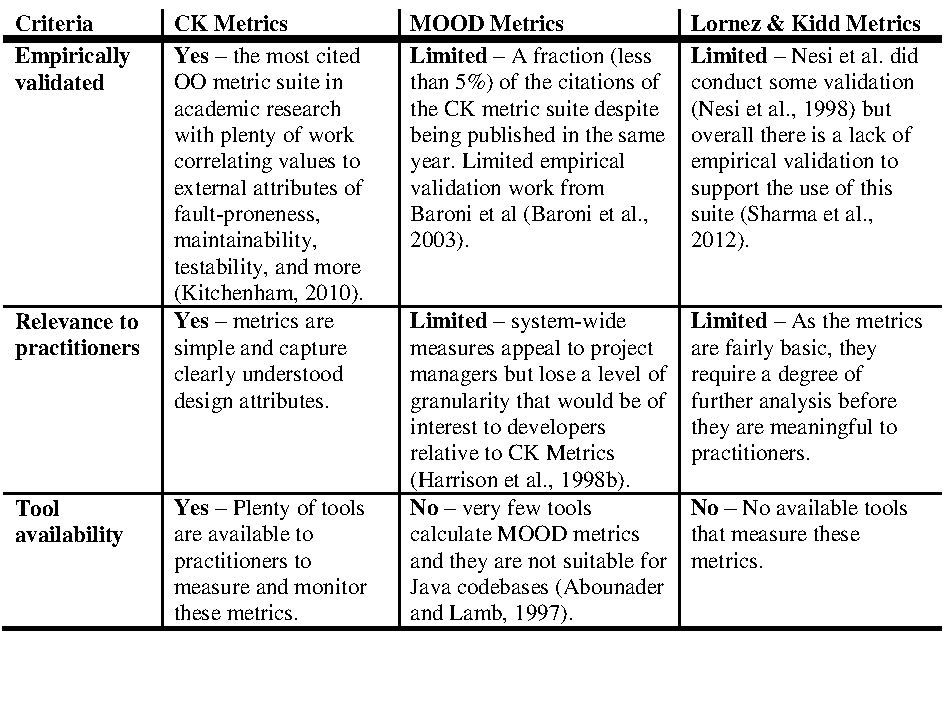
\includegraphics[width=1.0\textwidth]{MetricSuites.pdf}
 \label{tab:MetricSuites}
\end{tabular}
\end{table}